\section*{Wave–Vortex Duality and Swirl Momentum Conservation}
\addcontentsline{toc}{section}{Wave–Vortex Duality and Swirl Momentum Conservation}

Building on the fluid Hamiltonian formalism and the Jacobi energy structure, we now consider the conserved momentum in systems containing both distributed swirl and localized vorticity.

In stratified or rotating fluids, wavepackets induce a dipolar mean-flow response known as the Bretherton flow~\cite{buhler2005wave}. The impulse of this flow can be shown to equal the wavepacket’s integrated pseudomomentum. In such systems, the total conserved momentum takes the form:
\begin{equation}
    \frac{d}{dt} \left( \vec{P}_H + \vec{I} \right) = 0,
\end{equation}
where \( \vec{P}_H \) is the wave pseudomomentum and \( \vec{I} \) is the vortex impulse:
\begin{align}
    \vec{P}_H &= \int_V \vec{p} \, dV, \\
    \vec{I} &= \int_V \rho_\text{\ae} \, \vec{r} \times \vec{\omega} \, dV.
\end{align}

In the Vortex Æther Model, this conservation principle finds a natural reinterpretation. The pseudomomentum \( \vec{P}_H \) is replaced by the total swirl momentum stored in the distributed swirl field, written as:
\begin{equation}
    \vec{P}_\text{swirl} = \int_V \rho_\text{\ae} \, \nabla S(t) \, dV,
\end{equation}
where \( S(t) \) is the swirl clock phase satisfying \( \nabla S(t) = \vec{v}_\text{swirl} \).

The total ætheric impulse is thus:
\begin{equation}
    \frac{d}{dt} \left( \vec{P}_\text{swirl} + \vec{I}_\text{vortex} \right) = 0,
\end{equation}
with \( \vec{I}_\text{vortex} = \int \rho_\text{\ae} \, \vec{r} \times \vec{\omega} \, dV \) as the impulse of localized vortex knots.

This equation implies that swirl-phase propagation and vortex-core motion are two coupled aspects of a unified conservation law. The conventional quantum wave–particle duality is thus recast in VAM as a fluid-topological continuum:
\begin{center}
    \emph{Particles are not dual to waves; they are localized swirl states in a unified vortex medium.}
\end{center}
This formulation supports the broader VAM hypothesis that all observable dynamics emerge from conserved vorticity within an inviscid æther, eliminating the need for separate quantum or classical frameworks.



\section{Double-Slit Interference in the Vortex Æther Model}

The double-slit experiment, often cited as the definitive expression of wave–particle duality, presents no ontological paradox in the Vortex Æther Model (VAM). In standard quantum mechanics, interference arises even when individual quanta (e.g., electrons or photons) pass one at a time through two slits, suggesting they interfere with themselves. VAM resolves this not by invoking duality, but by recognizing each particle as a structured swirl entity with both localized and extended components.

Each vortex knot in VAM comprises:
\begin{itemize}[leftmargin=1.5em]
    \item A compact, knotted vortex core (the ``particle''),
    \item An extended, coherent swirl field \( \vec{\omega}(\vec{r}, t) \),
    \item A swirl phase clock \( S(t) = \int \Omega(r) \, dt \) that governs interference and coherence.
\end{itemize}

As a vortex knot approaches the slits, its core traverses one path, but its swirl phase field extends across both. The interference of these swirl contributions modulates the pressure field \( P(\vec{r}) \) in the æther:
\[
    \nabla P = -\frac{1}{2} \rho_\text{\ae} \nabla |\vec{\omega}|^2
\]
with:
\[
    \vec{\omega} = \vec{\omega}_1 + \vec{\omega}_2, \quad
    |\vec{\omega}|^2 = |\vec{\omega}_1|^2 + |\vec{\omega}_2|^2 + 2 \vec{\omega}_1 \cdot \vec{\omega}_2
\]

The resulting interference term governs the pressure landscape experienced by the core, which follows:
\[
    \frac{d\vec{r}_\text{core}}{dt} = -\frac{1}{\rho_\text{\ae}} \nabla P
\]

Thus, over many trials, a statistically weighted pattern emerges from deterministic guidance via the swirl interference field. No duality is needed: the wave-like and particle-like behavior arise from different aspects of the same vortex configuration.

This insight builds on the framework of wave–vortex duality developed in stratified fluids~\cite{buhler2005wave}, where wave packets induce dipole-like mean flows analogous to vortex impulse. In VAM, this equivalence is ontologized: all apparent quantum interference is the result of structured vorticity in an inviscid æther.



\section{Temporal Ontology and Phase Structure in VAM}

In the Vortex \AE ther Model (VAM), time is not a fundamental dimension but an emergent phenomenon tied to structured vorticity within the æther. This framework replaces the relativistic spacetime interval with a layered ontology of temporal modes, formally defined in the VAM Core Theory \cite{iskandarani2025vam2}. The present work extends that ontology by demonstrating how topological excitations encode distinct time signatures, swirlclock rates, and causal phases.

\subsection*{Temporal Layering}

We adopt the multi-modal structure of time described in \cite{iskandarani2025vam2}:
\begin{figure}[H]
    \centering
    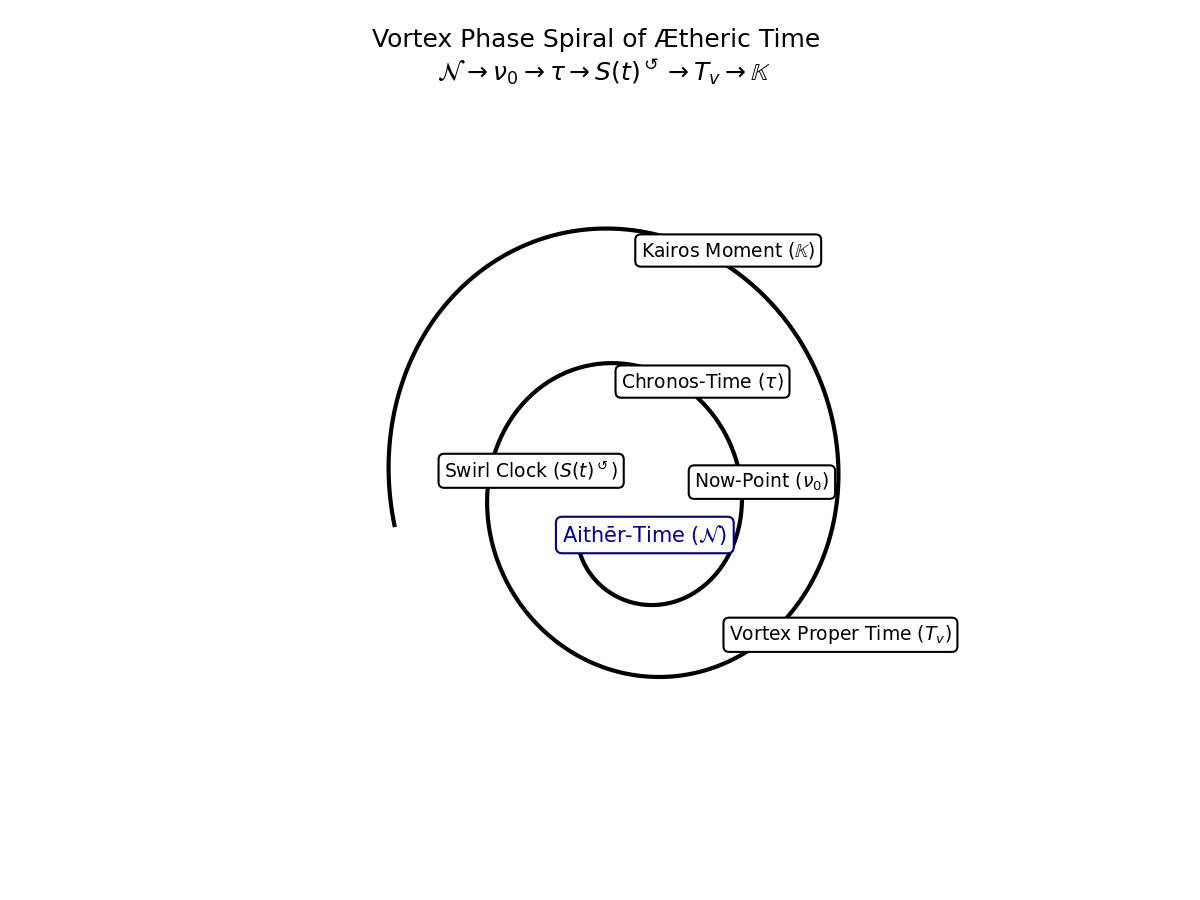
\includegraphics[width=0.7\textwidth]{images/TemporalOntologyv2}
    \caption{Temporal ontology in the Vortex Æther Model. Each layer represents a distinct phase of time, with the æther time $N$ as the absolute global parameter. The now-point $\nu_0$ defines local simultaneity, while observer time $\tau$ and swirlclock phase $S(t)$ emerge from structured vorticity.}
\end{figure}

\begin{table}[H]
\centering
\renewcommand{\arraystretch}{1.1}
\begin{tabular}{|l|l|l|}
\hline
\textbf{Symbol} & \textbf{Name} & \textbf{Interpretation} \\
\hline
$N$ & \textbf{Æther time} & Absolute global evolution parameter \\
$\nu_0$ & \textbf{Now-point} & Local simultaneity surface \\
$\tau$ & \textbf{Observer time} & Proper time: dependent on swirl density \\
$S(t)$ & \textbf{Swirlclock phase} & Emergent causal time: $\int \Omega_\text{swirl} dt$ \\
$T_v$ & \textbf{Vortex time} & Internal cycle time of knotted circulation \\
$\mathbb{K}$ & \textbf{Kairos moment} & Critical topological transition event \\
\hline
\end{tabular}
\caption{Temporal layers in the Vortex Æther Model (cf. Section 2.3 in \cite{iskandarani2025vam2}).}
\end{table}

\subsection*{Connection to Swirlclock Dynamics}

Our derivations of neutrino oscillations and $T$-violation are rooted in this ontology. In particular:

\begin{itemize}
    \item The \textbf{phase lag} $\Delta \theta_{ij}(t)$ between neutrino eigenstates directly corresponds to differential evolution in their local swirlclocks.
    \item The \textbf{vortex time} $T_v \sim 2\pi / \Omega_{\text{swirl}}$ defines the period of internal knot precession, replacing proper time in quantum oscillation models.
    \item The \textbf{observer time} $\tau$ is recovered via time dilation from vortex energy:
    \[
    d\tau = dt_\infty \sqrt{1 - \frac{U_{\text{vortex}}}{U_{\text{max}}}}, \quad
    U_{\text{vortex}} = \frac{1}{2} \rho_\text{\ae}^{(\text{energy})} |\vec{\omega}|^2.
    \]
    \item The \textbf{swirlclock-to-æther} conversion, valid across all energy scales, is:
    \[
    \frac{d\tau}{dN} = \sqrt{1 - \frac{v^2}{c^2}} \quad \text{(for uniform swirl speed)}
    \]
    or more generally,
    \[
    \frac{d\tau}{dN} = \sqrt{1 - \left( \frac{\vec{v} \cdot \vec{\omega}}{\omega_{\text{bg}} c} \right)^2},
    \]
    where $\omega_{\text{bg}}$ is the background swirl scale. This formulation links temporal flow to the energetics and orientation of vorticity fields.
\end{itemize}

This phase-based model of time aligns with the VAM temporal ontology defined over the manifold:
\[
N = E^3 \times N,
\]
where swirlclock phase $S(t)$ and vortex time $T_v$ represent emergent local and internal clock structures.

\begin{figure}[H]
    \centering
    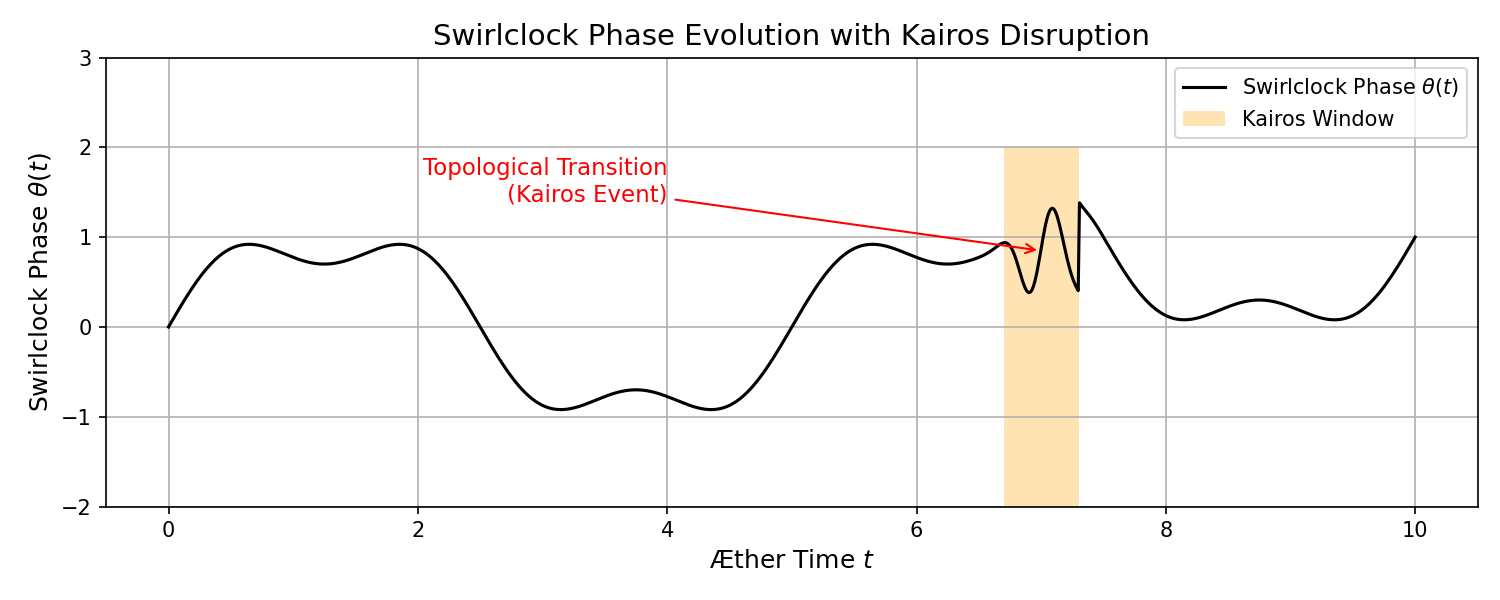
\includegraphics[width=0.7\textwidth]{images/TemporalOntologyKairosMoment}
    \caption{ Temporal ontology with Kairos moment $\mathbb{K}$ as a critical topological transition. This moment represents a discrete event where the swirlclock phase $S(t)$ and æther time $N$ align, marking a significant change in the system's state.}
\end{figure}

\subsection*{Topological Time Asymmetry}

The temporal asymmetry observed in kaon and neutrino oscillations becomes geometrically natural under VAM. Because mirror knots are not smoothly deformable into their counterparts under $T$-reversal:
\[
T: \theta(t) \rightarrow -\theta(-t),
\]
topological chirality introduces an intrinsic arrow of time. Matter--antimatter imbalance thus results not from arbitrary CP-violating phases but from topological swirlclock bias seeded during vortex formation in the early æther.

\subsection*{Conclusion}

This work aligns fully with the Temporal Ontology laid out in the foundational VAM documents. Swirlclock dynamics, topological chirality, and internal phase structure together yield an emergent model of time in which causal asymmetry, quantum oscillations, and gravitational dilation all arise from structured vorticity.

This lays the groundwork for a fully fluid-dynamical replacement of both spacetime curvature and complex Hilbert phase evolution in modern physics.
